%%%%%%%%%%%%%%%%%%%%%%%%%%%%%%%%%%%%%%%%%%%%%%%%%
% Signal region only fit studies. On Asimov dataset.
% OUTDATED
%%%%%%%%%%%%%%%%%%%%%%%%%%%%%%%%%%%%%%%%%%%%%%%%%
% \subsection{Signal region only fit}
% \label{app:boosted_fitstudies_SR}

% \begin{figure}[!h]
% \begin{center}
% \includegraphics*[width=1.00\textwidth]{./figures/boosted/SROnlyFit/40002000_NP_all}
% \caption{Pulls of nuisance parameters for the background-only likelihood fit to the background-only Asimov dataset in the signal region only.}
% \label{fig:boosted_fitstudies_SR_pullplot}
% \end{center}
% \end{figure}

% \begin{figure}[!h]
% \begin{center}
% 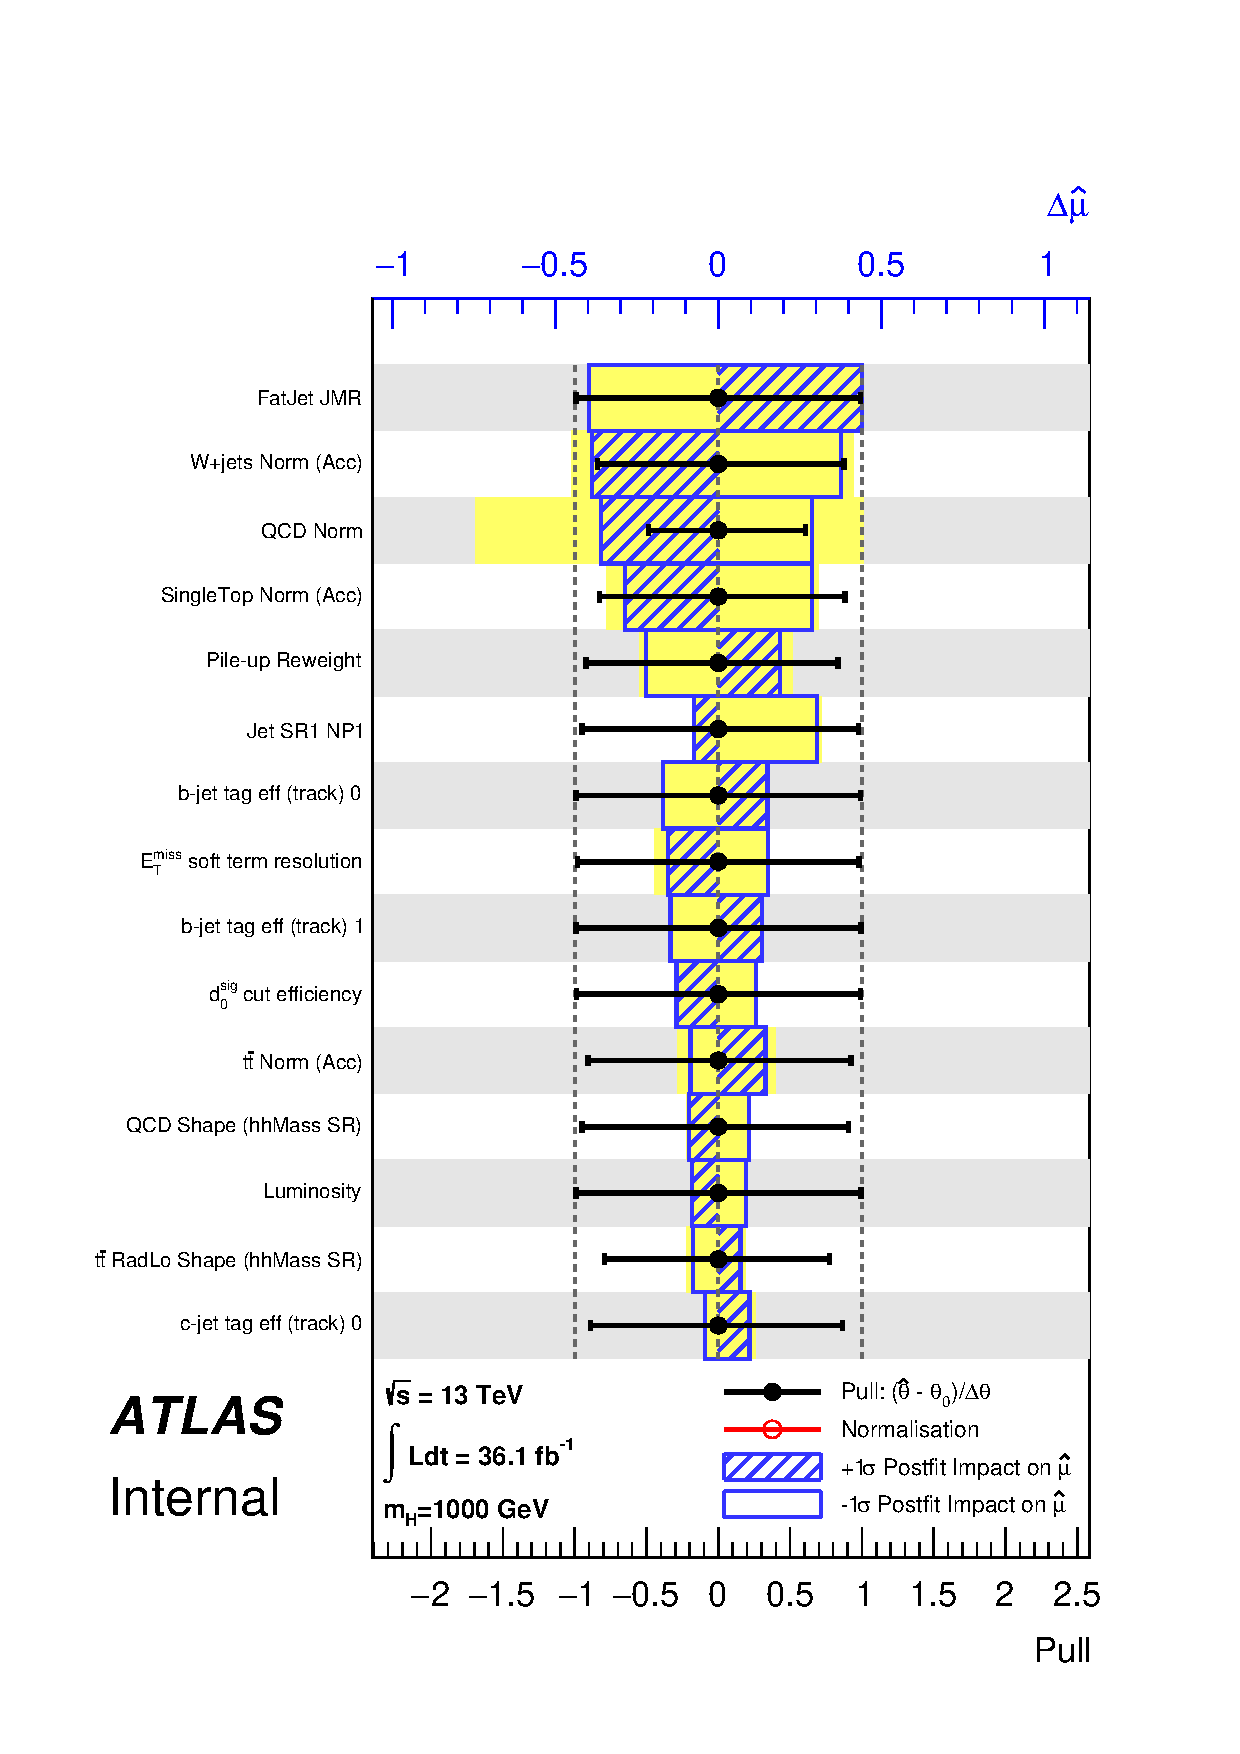
\includegraphics[scale=0.33]{./figures/boosted/SROnlyFit/40001000_Nominal_HH_13TeV_Nominal_Systs_SR_1000_pulls_1000}{fig:boosted_fitstudies_SR_ranking_1000}{$m_{H}$=1000~\GeV}
% 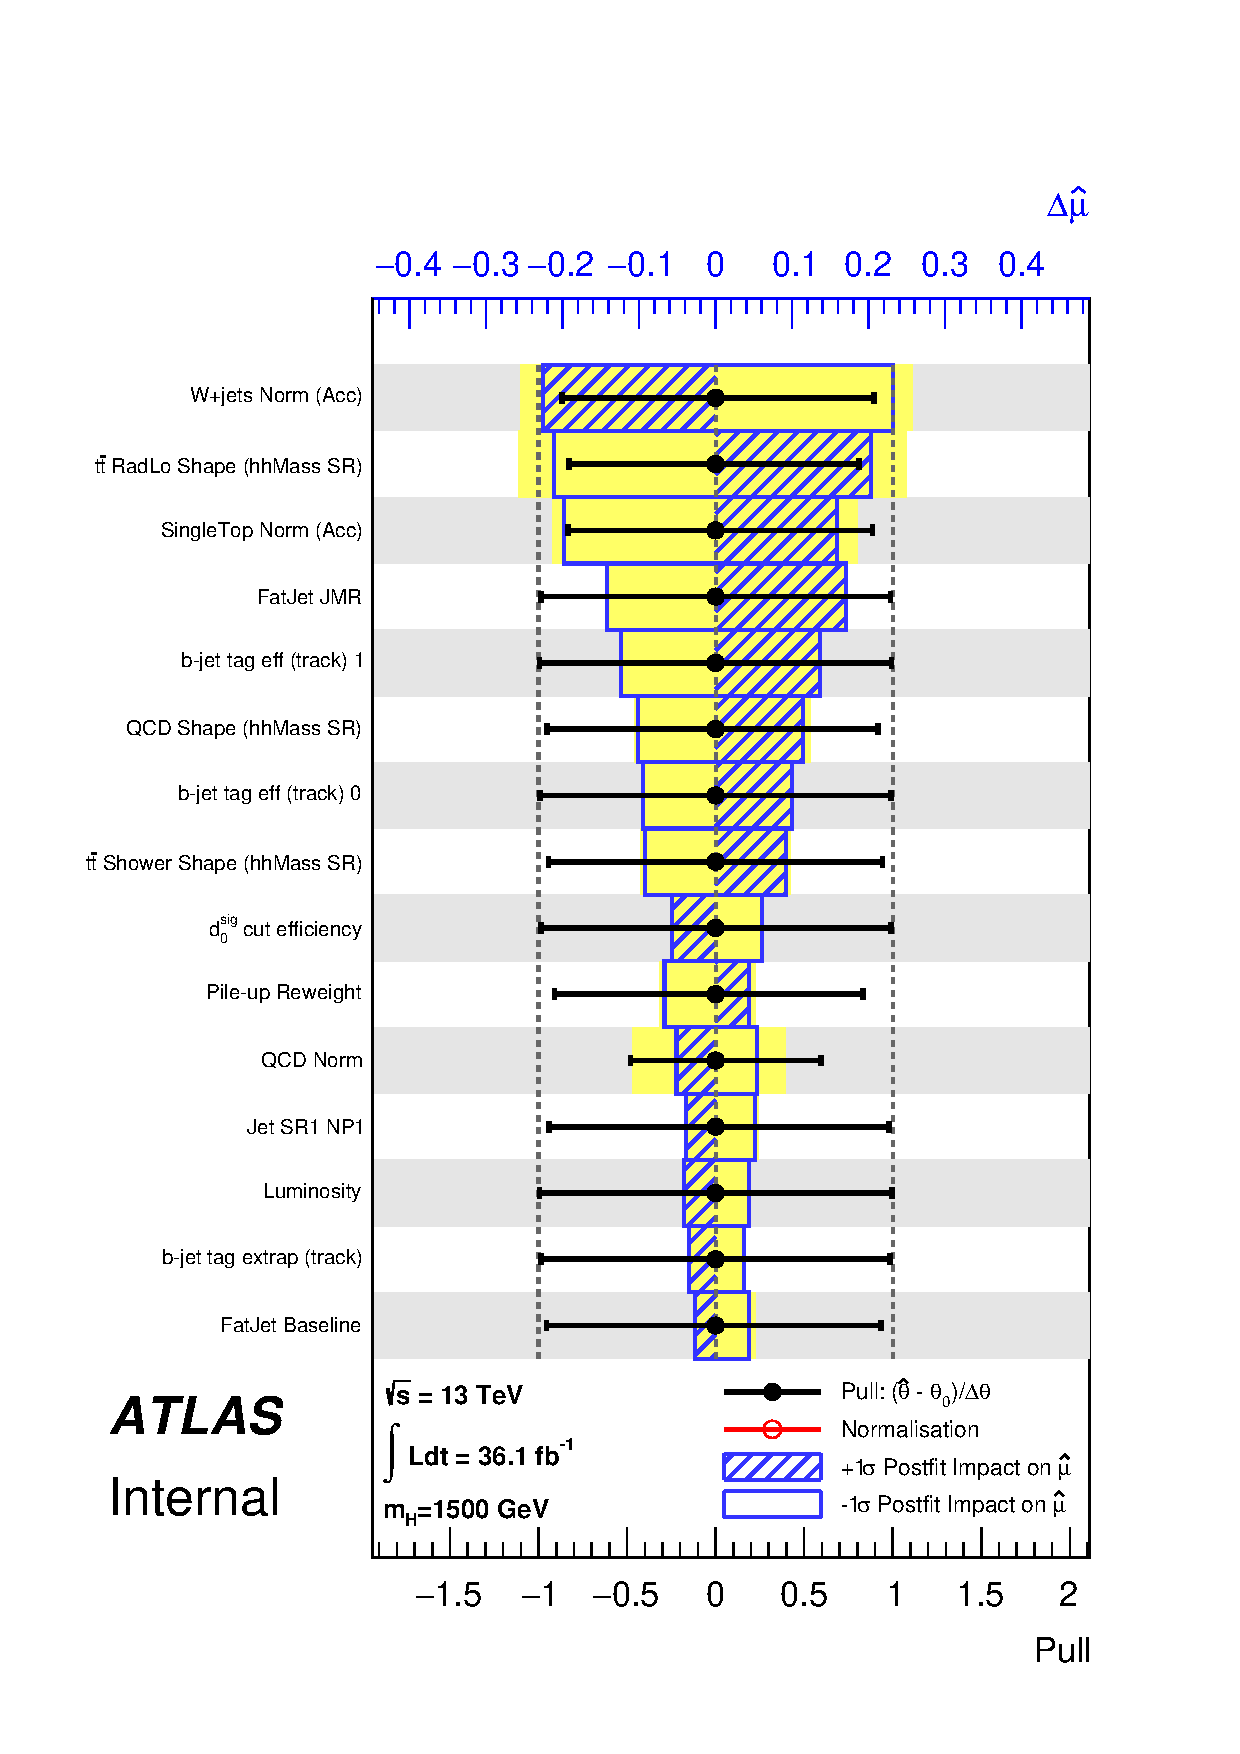
\includegraphics[scale=0.33]{./figures/boosted/SROnlyFit/40001500_Nominal_HH_13TeV_Nominal_Systs_SR_1500_pulls_1500}{fig:boosted_fitstudies_SR_ranking_1500}{$m_{H}$=1500~\GeV}\\
% 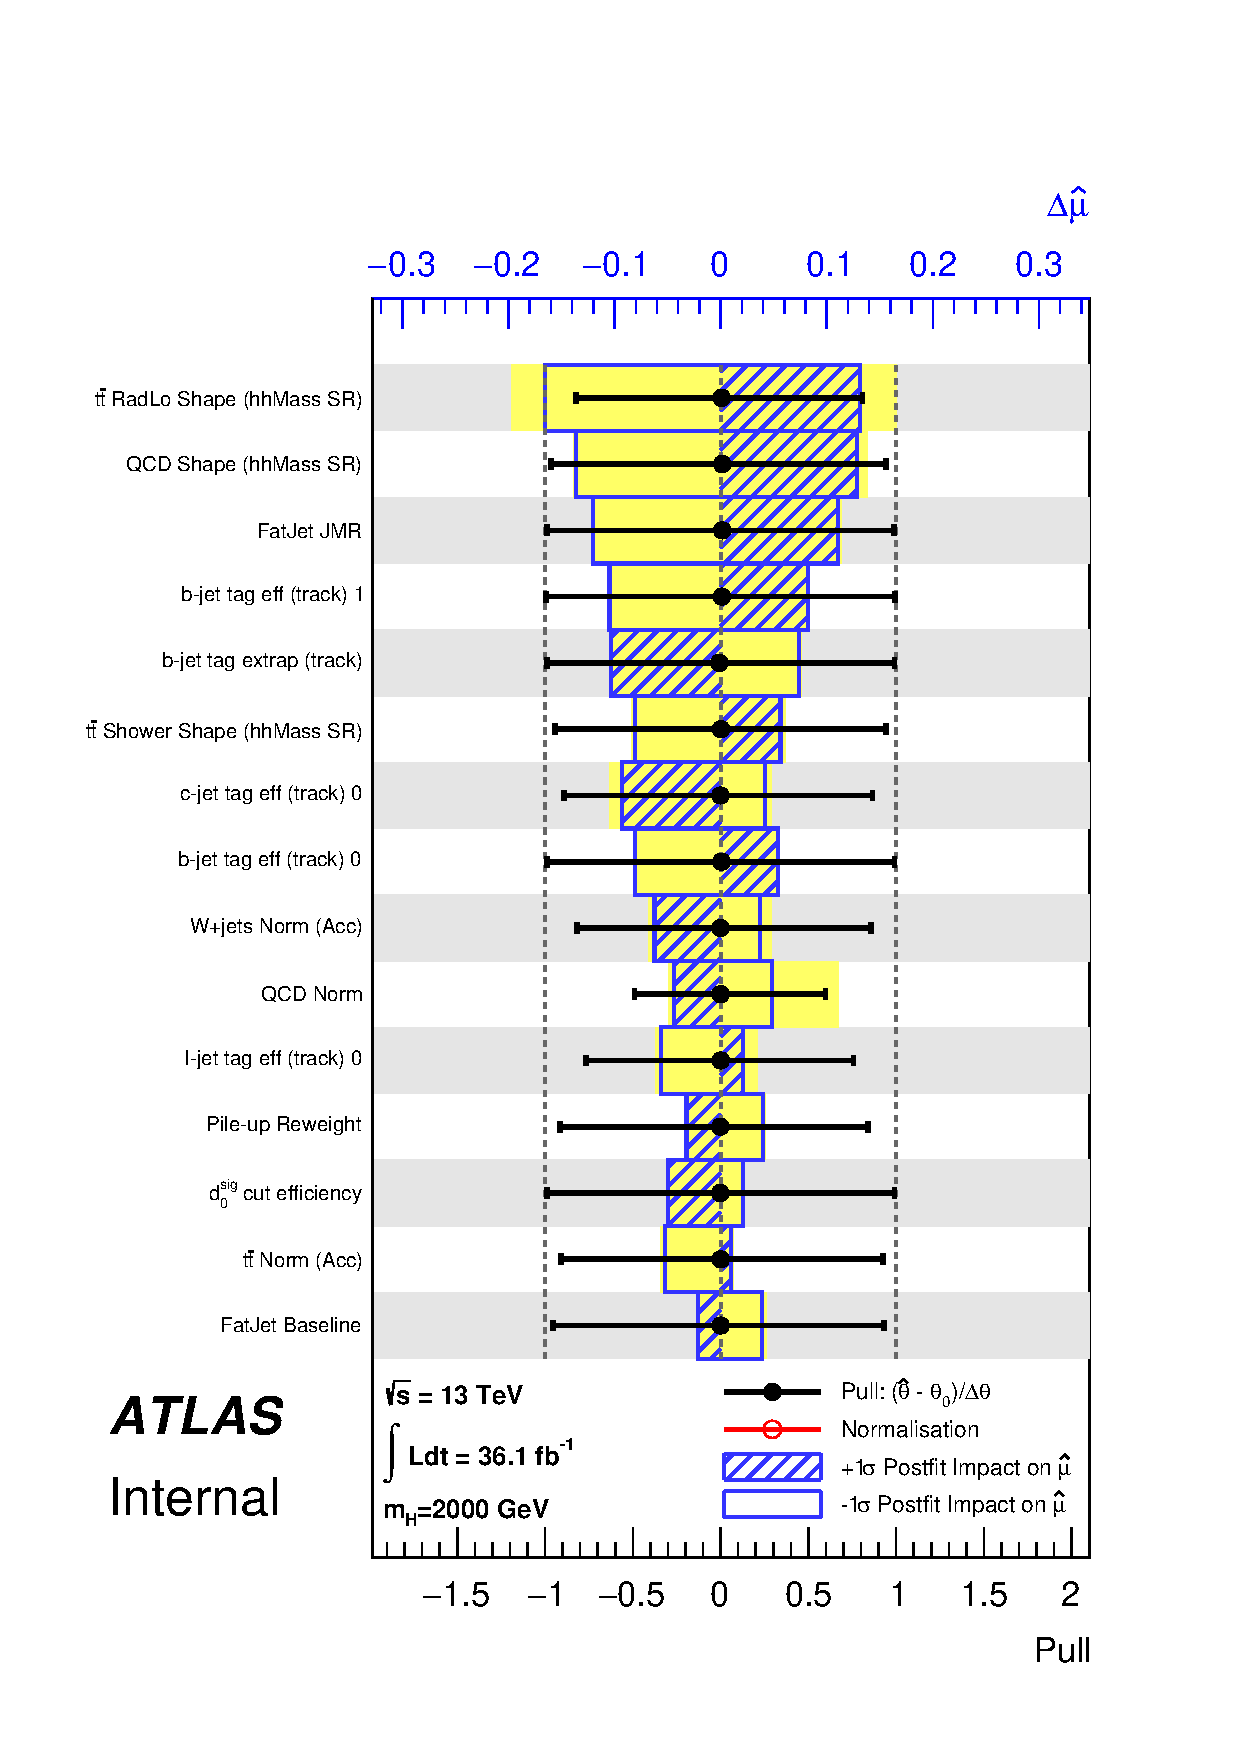
\includegraphics[scale=0.33]{./figures/boosted/SROnlyFit/40002000_Nominal_HH_13TeV_Nominal_Systs_SR_2000_pulls_2000}{fig:boosted_fitstudies_SR_ranking_2000}{$m_{H}$=2000~\GeV}
% 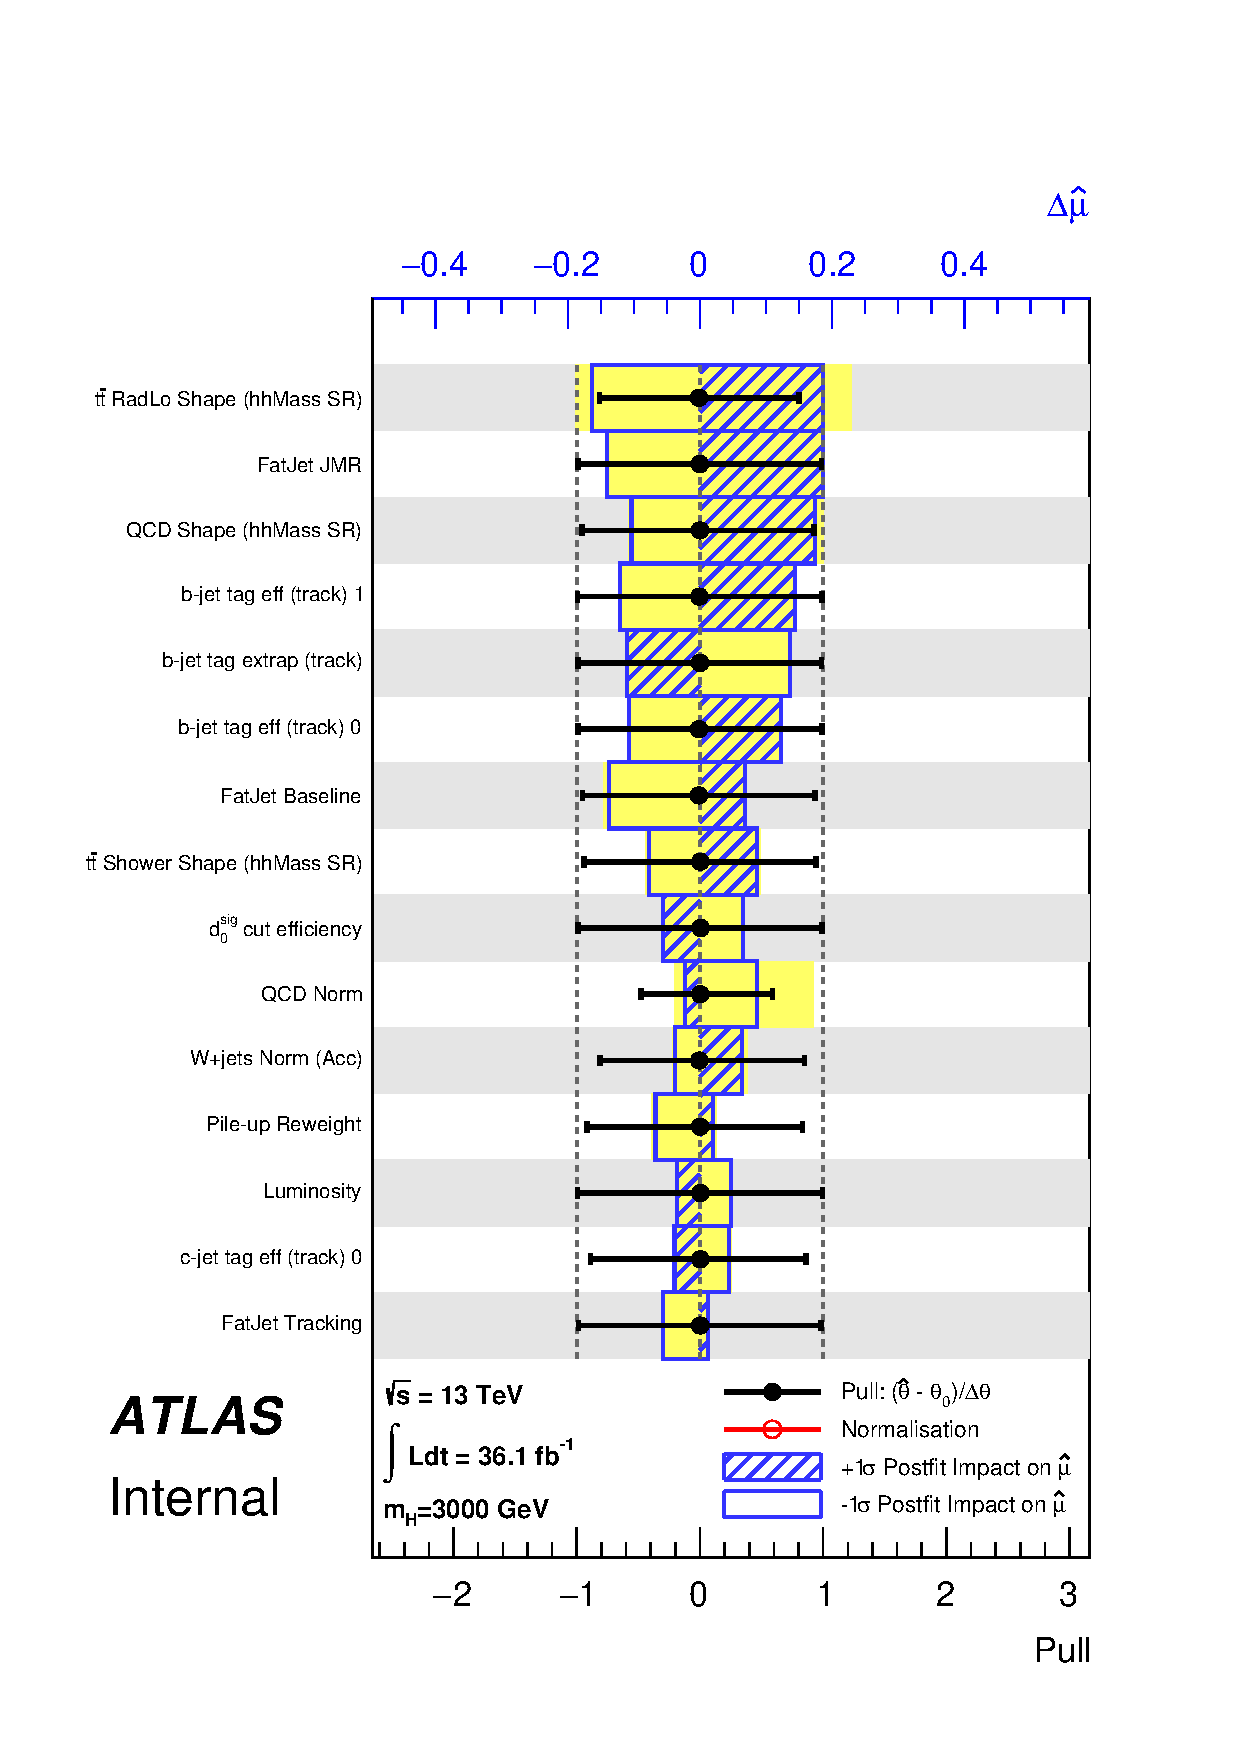
\includegraphics[scale=0.33]{./figures/boosted/SROnlyFit/40003000_Nominal_HH_13TeV_Nominal_Systs_SR_3000_pulls_3000}{fig:boosted_fitstudies_SR_ranking_3000}{$m_{H}$=3000~\GeV}
% \caption{Nuisance parameter ranking after the signal region only fit to the Asimov dataset for different signal resonance mass point of $m_{H}=$1000, 1500, 2000 
% and 3000~\GeV. The signal cross-sections for each signal mass points are normalized to their expected upper limit. 
% The nuisance parameters are ranked according to its postfit impact (blue band) on $\hat{\mu}$. The yellow band corresponds to the prefit impact.}
% \label{fig:boosted_fitstudies_SR_ranking}
% \end{center}
% \end{figure}

% \begin{figure}[!h]
% \begin{center}
% \includegraphics*[width=1.00\textwidth]{./figures/boosted/SROnlyFit/40002000_corr_origin}
% \caption{Correlation matrix of nuisance parameters in the likelihood fit after the conditional $mu$=0 fit of the $m_{hh}$ distribution 
% in the signal region.}
% \label{fig:boosted_fitstudies_SR_corrmatrix_1}
% \end{center}
% \end{figure}

% \begin{figure}[!h]
% \begin{center}
% \includegraphics*[width=1.00\textwidth]{./figures/boosted/SROnlyFit/40002000_corr_HighCorr}
% \caption{Correlation matrix of nuisance parameters in the likelihood fit after the conditional $mu$=0 fit of the $m_{hh}$ distribution 
% in the signal region. Nuisance parameters with correlation factor of larger than 10\% are shown.}
% \label{fig:boosted_fitstudies_SR_corrmatrix_1}
% \end{center}
% \end{figure}

% \clearpage
% \FloatBarrier

%%%%%%%%%%%%%%%%%%%%%%%%%%%%%%%%%%%%%%%%%%%%%%%%%
% Signal region only fit studies with a single bin. 
% On Asimov dataset.
% 
%%%%%%%%%%%%%%%%%%%%%%%%%%%%%%%%%%%%%%%%%%%%%%%%%
\subsection{Single bin fit}
\label{app:boosted_fitstudies_SR_singlebin}

\begin{figure}[!h]
\begin{center}
\includegraphics*[width=1.00\textwidth]{./figures/boosted/SROnlyFitOneBin/NP_allExceptGammas}
\caption{Pulls of nuisance parameters for the fit to the background only Asimov dataset in the signal region only fit using a single bin histogram,
effectively it is a counting experiment fit.}
\label{fig:boosted_fitstudies_SRsinglebin_pullplot}
\end{center}
\end{figure}

\clearpage
\FloatBarrier


%%%%%%%%%%%%%%%%%%%%%%%%%%%%%%%%%%%%%%%%%%%%%%%%%
% mBB control region fit studies On Asimov dataset.
% OUTDATED
%%%%%%%%%%%%%%%%%%%%%%%%%%%%%%%%%%%%%%%%%%%%%%%%%
\subsection{mBB control region only fit}
\label{app:boosted_fitstudies_mBBcr}

In this section we study the mBB control region only fit. In this fit exercise, the $t\bar{t}$ and W+jets background normalization 
are allowed to float and determined from the mBB control region fit to the large-$R$ jet mass distribution. The jet mass distribution is chosen
as the fitted distribution due to the fact that the low jet mass region is relatively enriched with W+jets events with respect to the 
high jet mass region where it is predominantly consists of $t\bar{t}$ events as shown in Figure~\ref{fig:mBBcr_mBB_prefit}.

Table~\ref{tab:boosted_fitstudies_mBBcr_normfact} shows the calculated normalization factors from the from the mBB control
region only fit of the large-$R$ jet mass distribution to the observed data. Figure~\ref{fig:mBBcr_mBB_postfit} shows 
the large-$R$ jet mass distribution after the fit and it can be seen that the agreeement between the total background
and the observed data is now improved. Table~\ref{tab:boosted_bkgd_mbbcr_yields_postfit} shows the postfit yields for
each background and the total background in the mBB control region. Figure~\ref{fig:boosted_fitstudies_mBBcr_pullplot} shows the 
pull of the nuisance parameters in the fit to the background-only Asimov dataset and to the observed data. 
 
\begin{figure}[!h]
\begin{center}
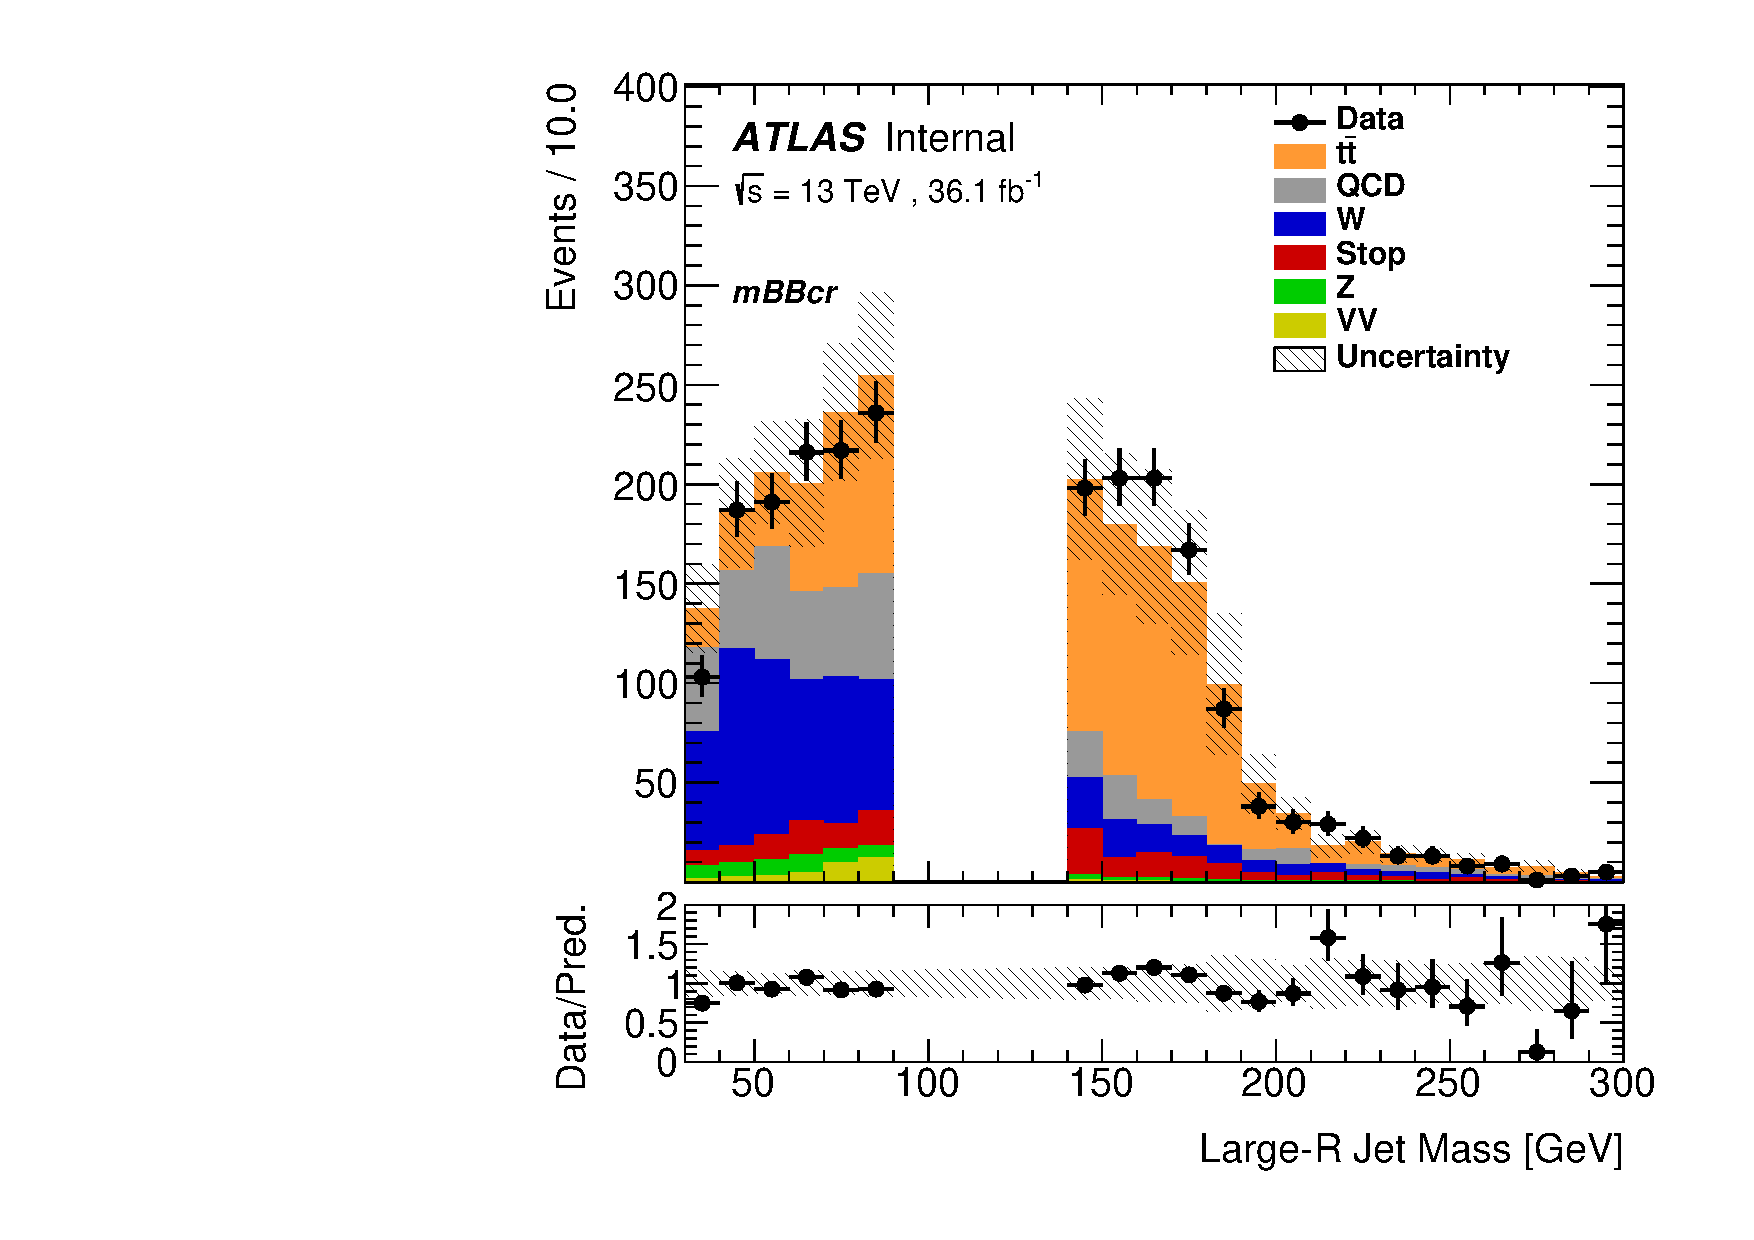
\includegraphics[scale=0.33]{./figures/boosted/CROnlyFit/mBB_Prefit}
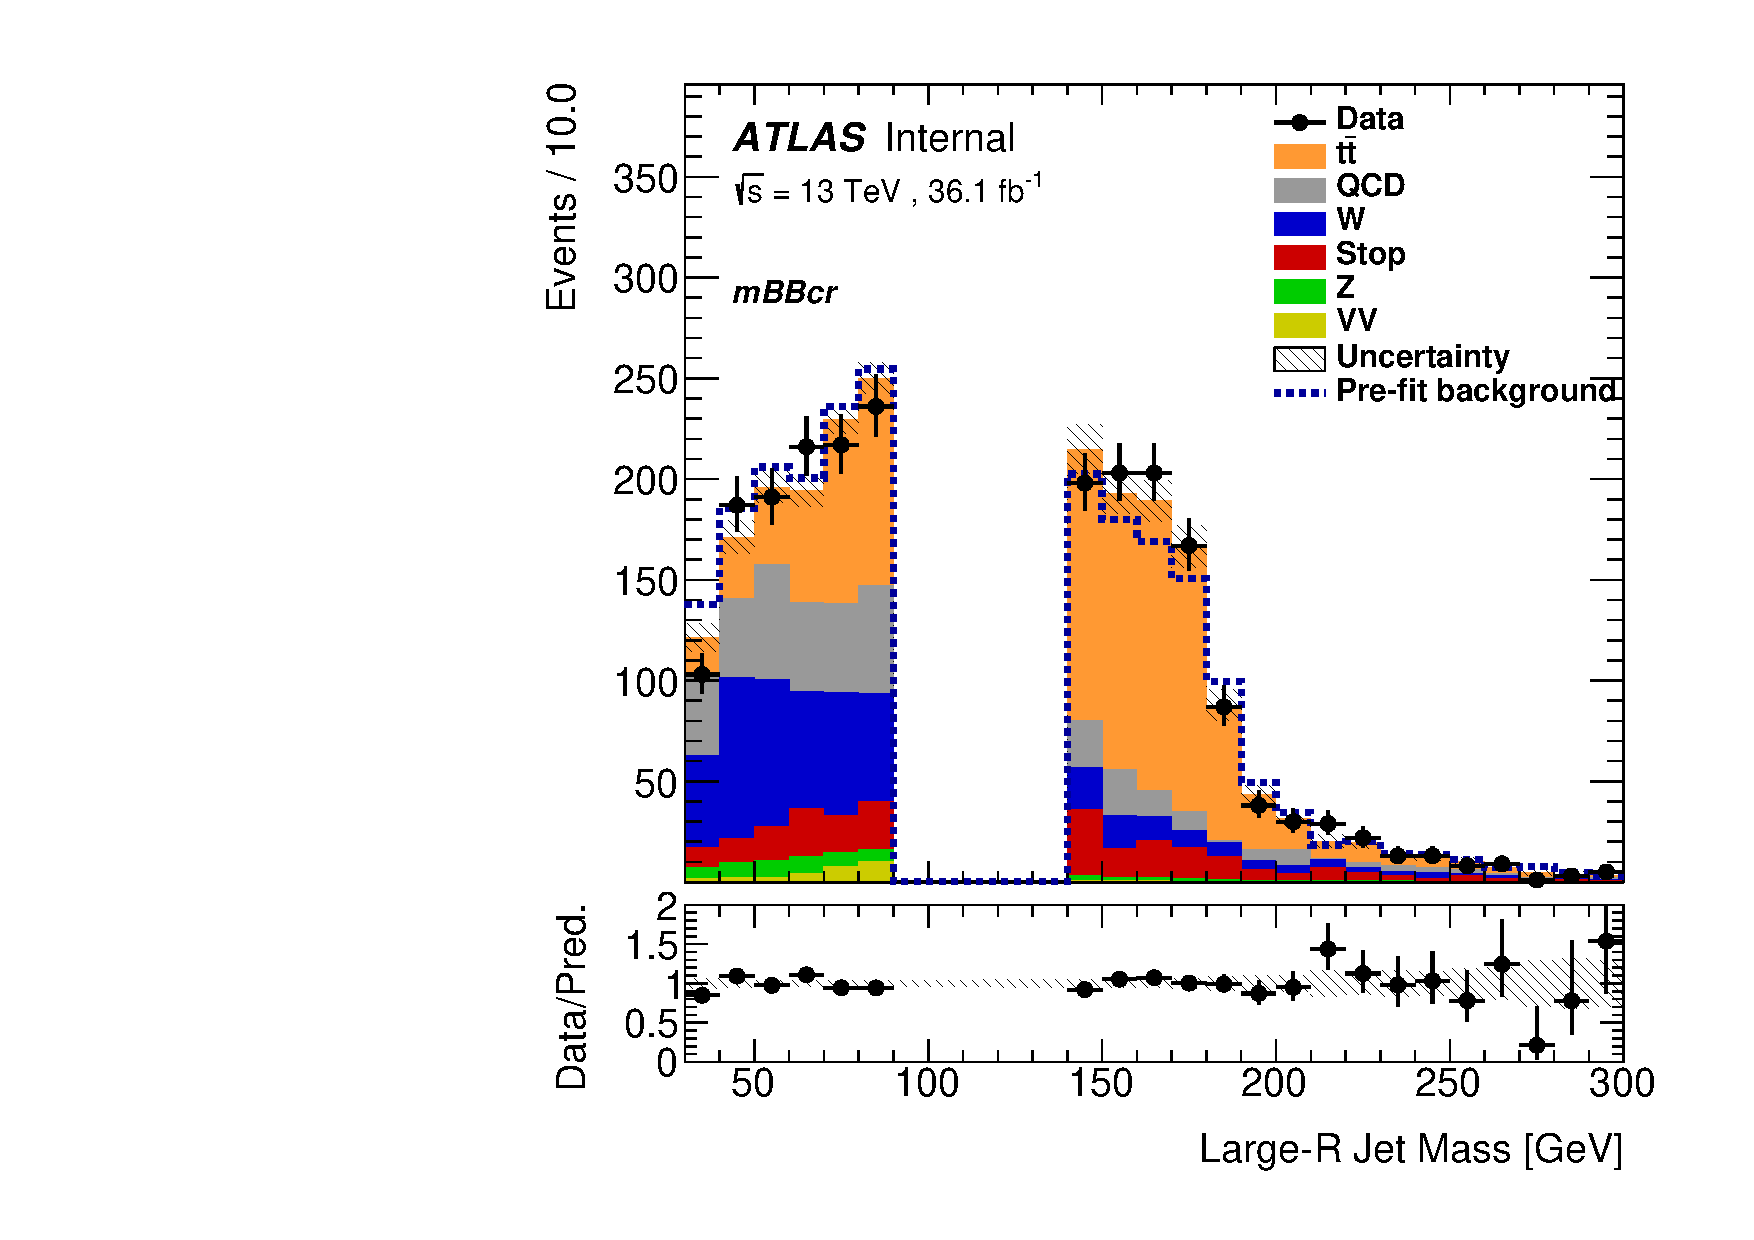
\includegraphics[scale=0.33]{./figures/boosted/CROnlyFit/mBB_Postfit}\\
\caption{Prefit and postfit large-$R$ jet mass distribution in the mBB control region only fit.}
\label{fig:boosted_fitstudies_mBBcr_mBB}
\end{center}
\end{figure}

\begin{table}
\begin{center}
\begin{tabular}{c|c}
Background & Normalization factor  \\      
\hline
$t\bar{t}$ &  0.941 $\pm$ 0.212 \\
W+jets     &  1.032 $\pm$ 0.243 \\
\end{tabular}
\end{center}
\caption{Normalization factors for $t\bar{t}$ and W+jets backgrounds calculated from the mBB control
region only fit of the large-$R$ jet mass distribution to the observed data.} 
\label{tab:boosted_fitstudies_mBBcr_normfact}
\end{table}

\begin{table}
\begin{center}
\begin{tabular}{l|c|c} 
Sample        &    Yield &  Stats+Systs \\ 
\hline 
$t\bar{t}$    &  1035.0  & - \\ 
W+Jets        &  459.9   & - \\ 
QCD           &  376.27  & - \\ 
Single-top    &  225.86  & - \\ 
Z+Jets        &  55.05   & - \\ 
Dibosons      &  31.52   & -  \\ 
\hline 
Prediction    &  2183.7  &  56.71 \\ 
Data          &  2179    &  -\\ 
\hline 
Data/Pred     &  1.00    &  \\ 
\hline 
\end{tabular} 
\end{center}
\caption{Postfit background yields and observed data yields in the mBB control region.}
\label{tab:boosted_bkgd_mbbcr_yields_postfit}
\end{table}


\begin{figure}[!h]
\begin{center}
\includegraphics*[width=1.00\textwidth]{./figures/boosted/CROnlyFit/NP_allExceptGammas}
\caption{Pulls of nuisance parameters for the fit to the background only Asimov dataset (red) 
and to the observed data (black) in the mBB control region only fit.}
\label{fig:boosted_fitstudies_mBBcr_pullplot}
\end{center}
\end{figure}

